\documentclass[12pt,twoside]{report}
\usepackage[utf8]{inputenc}
\usepackage{graphicx}
\usepackage{caption}
\usepackage{subcaption}
\usepackage{setspace}
\graphicspath{ {./images/} }
% determime the page layout + allow the inclination of even and odd page are the same.
\usepackage[a4paper,width=150mm,top=25mm,bottom=25mm,bindingoffset=6mm]{geometry}
\usepackage{emptypage}  % Ensures no headers or footers on empty pages

\usepackage{listings}
\usepackage{amsmath}
\usepackage{enumitem}
\usepackage{varwidth}
\usepackage{tasks}

\usepackage[style=alphabetic]{biblatex}
\addbibresource{references.bib}

\usepackage{tikz}
\usetikzlibrary{calc}
\usetikzlibrary{positioning}
\usetikzlibrary {shapes.geometric}


\usepackage{fancyhdr}
\pagestyle{fancy}
\setlength{\headheight}{14.49998pt}

% Initial fancyhdr setup
\fancyhead{}
\fancyhead[RO,LE]{Thesis Title}
\fancyfoot{}
\fancyfoot[LE,RO]{\thepage}
\fancyfoot[LO,CE]{Chapter \thechapter}
\fancyfoot[CO,RE]{Author Name}
\renewcommand{\headrulewidth}{0.4pt}
\renewcommand{\footrulewidth}{0.4pt}

\begin{document}
\begin{titlepage}
  \begin{center}
  \begin{tikzpicture}[remember picture, overlay]
    \draw [line width=1pt]
        ($ (current page.north west) + (1.5cm,-2.0cm) $)
      rectangle
      ($ (current page.south east) + (-1.5cm,1.8cm) $);
    
  \end{tikzpicture}

  \begin{figure}[htbp]
    \begin{minipage}{0.5\linewidth}
    \centering
    
\includegraphics[width=\textwidth]{vgu_logo.jpg}
    \end{minipage}
    \hfill{\hspace{2cm}}
    \begin{minipage}{0.4\textwidth}
    \centering
    
\includegraphics[width=\textwidth]{FRA-UAS.png}
    \end{minipage}
    \end{figure}

    \vspace*{1cm}

    \textbf{\large \uppercase{vietnamese - german university}}

    \vspace*{0.5cm}

    \uppercase{\large Department of computer science}

    \vspace*{1cm}

    \textbf{Frankfurt university of applied sciences}

    \vspace*{0.5cm}

    Faculty 2: Computer Science and Engineering

    \vspace{1cm}

    \textbf{\LARGE 
    Evaluation And Implementation of}
    \vspace{0.3cm}

    \textbf {\LARGE Modern Virtual Private Network }

    \vspace{0.3cm}
    \textbf{\LARGE Protocol for The GNRC Network Stack}

    \vspace{0.8cm}
    \large By
    \vspace{0.2cm}

    \large Le Hoang Dang Nguyen
    \vspace{0.2cm}

    \large Matriculation number: 17028

    \vspace{0.7cm}
    \textbf{\uppercase{Bachelor Thesis}}

    \vspace{0.7cm}
    Submitted in partial fulfillment of the requirements for the degree of 
    Bachelor Engineering in study program Computer Science, Vietnamese - German University, 2024
    \vspace{1cm}

      \textbf{First supervisor:} Prof. Dr. Oliver Hahm \\
      \textbf{Second supervisor:} Dr. Tran Thi Thu Huong

    \vfill

    Binh Duong, 2024

  \end{center}
\end{titlepage}

\newpage  % Start a new page
\thispagestyle{empty}  % Suppress headers and footers
\hbox{}  % Empty box to position text
\vfill  % Vertically center the content
\begin{center}
\Large This page intentionally left blank.
\end{center}
\vfill  % Fill the rest of the page vertically

\newpage  % Start a new page after the blank one

\chapter *{\centering Declaration}
\doublespacing
\large I hereby declare that this thesis is a product of my own work, unless
otherwise referenced. I also declare that all opinions, results, conclusions
and recommendations are my own and may not represent the policies or
opinions of Vietnamese – German University.

\vspace{12cm}  % Space above the signature line

\noindent\hfill\rule{8cm}{0.4pt}  % Right-aligned line for the signature
\vspace{0.5cm} % Space between the line and the name

\noindent\hspace{8cm} Le Hoang Dang Nguyen % Right-aligned line for the signature

\chapter*{\centering Acknowledgements}
I want to thank you.

\chapter*{\centering Abstract}
Abstract go here

\tableofcontents

\chapter{Introduction}
\section{Motivation}
  The modern world is showing great interest in the \gls{iot} with the expectation
  of a significant increase in the number of the internet-connected devices \cite{things}. In 2016, forecasts by 
  Statista estimated that there would be more than 75 billions \gls{iot} devices in used \cite{stat}. 
  However, this rapid, unregulated expansion also comes with serious privacy and security challenges \cite{chals}.
  One such vector of security attack could be the router, the machine standing between the \gls{iot}
  devices and the internet. In 2018, Cisco researcher found out a new malware called VPNFilter
  affecting 500,000 networking devices worldwide, including Mikrotic routers \cite{router}. 
  With such a malware, the hackers may have the ability to hijack any traffic between
  the device and the internet outside. Thus, better security mechanisms need to be enforce
  to guarantee an end-to-end (E2E) secure communication of the \gls{iot} devices against such
  untrustworthy actors.

  \gls{vpn} could possibly be one of the approachs. \gls{vpn} does not only 
  ensure the encryption of network traffic, but also hides away the original addresses coming
  from the devices, making network communication private to only the owners. However, adapting
  normal \gls{vpn} technology for \gls{iot} devices faces serious physical limitation of such devices.
  These devices are usually small, with severe constraints on power, memory, 
  and processing resources \cite{rfc7228}. On the otherhand, existent \gls{vpn} protocols like OpenVPN or 
  IPSec are complex, fragile against faulty misconfiguration and have many known vulnerabilites \cite{pwu}. 
  There has been recent effort on adapting IPSec protocol for the constrained enviroments by
  reducing the requirements for an implementation to the minimum \cite{rfc9333} and developing
  a compression framework for the protocol \cite{ietf-ipsecme-diet-esp-01}. 

  Another consideration to introduce the \gls{vpn} into the \gls{iot} infrastructure is Wireguard \cite{wireguard}.
  Wireguard is a modern \gls{vpn} protocol designed for Linux with simplicity and security in mind.
  While achive multiple security properites, the Wireguard messages still has low overhead 
  and a potential low memory footprint, making it desirable for the class of constrained devices.

  The goal of this thesis is to evaluate the merits that Wireguard can bring into the Internet
  of Things fields and propose an implementation of the protocol for GNRC - a network stack designed
  specifically for the \gls{iot} enviroment.

\section{Organization}
  The thesis is organized as follows:
  \begin{itemize}
    \item Chapter \ref{chap:wei} provides the background knowlegde of \gls{iot}, Wireless embedded internet and
    \gls{6lowpan}.
    \item Chapter \ref{chap:gnrc} gives an overview on the GNRC network stack, and RIOT operating
    system that runs on top of it.
    \item Chapter \ref{chap:wireguard} explains in details the Wireguard protocol.
    \item Chapter \ref{chap:eval} describes the security features of Wireguard and evaluate
    the benefits they can add to the Internet of Things.
    \item Chapter \ref{chap:des} focuses on the design and important implementation apsects of
    Wireguard for GNRC.
    \item The final chapter concludes and summarizes the main works of the thesis.
  \end{itemize}
\chapter{Wireless Embedded Internet} \label{chap:wei}

This chapter provide the definition and overview of the wireless embedded internet. It covers
It covers architectures specifically developed for IoT applications, hightlights the \gls{6lowpan}
protocol stack that allows the integration of the \gls{ip} stack onto this type
of network, and reviews 802.15.4, a common protocol in embedded context.

\section{Overview}
The Internet of Things (IoT) comprises of all embedded devices and networks that are natively 
\gls{ip}-enabled and connected to the Internet, such as sensors, machines, and \gls{rfid} readers, 
alongside the services monitoring and controlling these devices \cite{wie}. A subset of \gls{iot}, 
the Wireless Embedded Internet consists of low-power, resource-limited wireless devices 
connected through standards like IEEE 802.15.4. Integrating standard Internet protocols with such networks 
presents several challenges:

\begin{description}
  \item[Power and duty-cycle:] The IP-enabled devices should always be connecting, contradicting the low-duty-cycle
 nature of the battery-powered wireless devices.
  \item[Multicast:] Wireless embedded radio technologies like IEEE 802.15.4, do not generally support multicast, and
 flooding wastes power and bandwidth in such network. However, Multicast is an important operation
 for many IPv6 features such as address auto-configuration \cite{rfc4862}. 
  \item[Limited bandwidth and frame sizes:] Bandwith and frame size inside a low-power wireless embedded radio network
 are limited, with only 20-250 kbits/s and 40-200 bytes correspondingly. For example, the frame size 
 for IEEE 802.15.4 standard has a 127-byte frame size, with layer-2 payload sizes as low as 72 bytes. The minimum
 frame size for standard IPv6 is 1280 bytes \cite{rfc8200}, hence fragmentation is required.
  \item[Reliability:] Standard Internet Protocols are not optimized for low-power wireless networks. For
 example, TCP is not able to differentiate between packets dropped by congestion or lost on wireless links.
 Node failure, energy exhaustion, and sleep duty cycles can also incur unreliability in wireless embedded networks.
\end{description}

 To tackle these issues, 6LoWPAN \cite{rfc4944} was developed, enabling IPv6 and its related protocols 
 to function effectively in wireless embedded networks. IPv6’s simple header structure 
 and hierarchical addressing make it ideal for use in these constrained environments.

\section{The 6LoWPAN Architecture}
  According to Zach Shelby and Carsten Bormann, the Wireless Embedded Internet 
  is formed by connecting islands of wireless embedded devices, 
  with each island functioning as a stub network within the Internet \cite[p.~13]{wie}. 
  A stub network is one where IP packets are either sent to or received from, 
  but it does not serve as a transit point for other networks. The 6LoWPAN architecture is
  illustrated in Figure \ref{fig:lowpan}. In this context, the 6LoWPAN architecture consists of low-power wireless area networks (LoWPANs), 
  which operate as IPv6 stub networks. Each LoWPAN is a set of 6LoWPAN nodes, sharing a common
  IPv6 address prefix (the first 64 bits of an IPv6 address), with the interconnection between the
  LoWPANs achieved through the edge router. There are 3 different kinds of LoWPANs:
  \begin{itemize}
    \item An \textbf{Ad hoc LoWPAN} operates independently without the connection to the internet.
    \item A \textbf{Simple LoWPAN} connects to another IP network via an edger router.
    \item An \textbf{External LoWPAN} comprises LoWPANS of multiple edge routers along
    with a backbone link connecting them.
  \end{itemize}

  \begin{figure}[h]
    \centering
    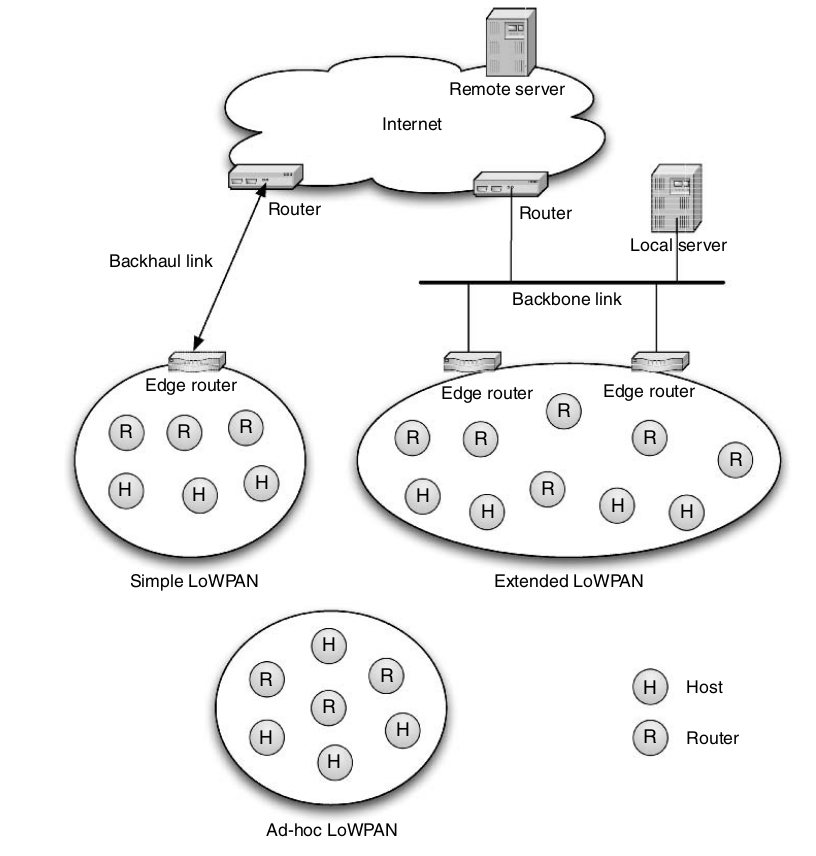
\includegraphics[width=0.8\linewidth]{lowpan}
    \caption{The 6LoWPAN architecture, see \cite[p.~14]{wie}}
    \label{fig:lowpan}
  \end{figure}

  LoWPANs are connected to other IP networks via edge routers, as illustrated in Figure 
  \ref{fig:lowpan}. The edge router plays a key role by routing traffic to and from the LoWPAN, 
  managing 6LoWPAN  compression, handling Neighbor Discovery within the network, and other network
  management features. Each node in a LoWPAN could either be a host, an edge router, or a node routing
  between other nodes. The shared common IPv6 prefix within the LoWPAN is advertised by edge routers
  or is pre-configured on each node. An edge router keeps a list of registered nodes that are accessible 
  through its network interface inside the LoWPAN.

  To enter a 6LoWPAN, a node sends a Router Solicitation message to obtain the IPv6 prefix unless it
  has been statically configured. Upon receiving the prefix, the node generates a unique global IPv6 
  address and registers this address with the edge router of the LoWPAN. This allows the edge router 
  to make informed routing decisions for traffic entering and exiting the LoWPAN, as well as to 
  facilitate neighbor discovery within the 6LoWPAN. The edge router must update the list of registered 
  nodes regularly, as addresses expire after a configurable period.  A longer expiration time 
  helps reduce a node's power consumption, while a shorter expiration time accommodates rapidly 
  changing network structures. These processes are defined in the dedicated neighbor discovery
  protocol for 6LoWPAN \cite{rfc6775}. LoWPAN nodes can travel freely within and among multiple 
  LoWPAN networks, and they may participate in several LoWPANs simultaneously. Communication 
  between a LoWPAN node and an external IP node occurs in an end-to-end manner, similar to 
  interactions between standard IP nodes.

  In an extended LoWPAN, multiple edge routers are integrated into the same LoWPAN, 
  sharing the same IPv6 prefix. These edge routers are interconnected through a common backbone link. 
  When a node moves between edge routers, it must register with the edge router it can access, 
  but it retains its IPv6 address. Communication between edge routers regarding neighbor 
  discovery is handled over the backbone link, which reduces messaging overhead. 
  This extended LoWPAN architecture allows a single LoWPAN to cover larger areas.

  An ad-hoc LoWPAN works in the same manner as a simple LoWPAN, but without the link to other
  IP networks. Instead of an edge router, a node will act as a simple edge router, handle unique 
  local address generation \cite{rfc4193} and provide the neighbor discovery registration feature 
  to other nodes.

\section{6LoWPAN Protocol Stack}
  Figure \ref{fig:ip_vs_low} depicts the IPv6 protocol stack with 6LoWPAN in comparison to a standard IP protocol 
  stack and the corresponding five layers of the Internet model. This Internet model 
  connects a wide range of link-layer technologies with various transport and application protocols.

  \begin{figure}[h]
    \centering
    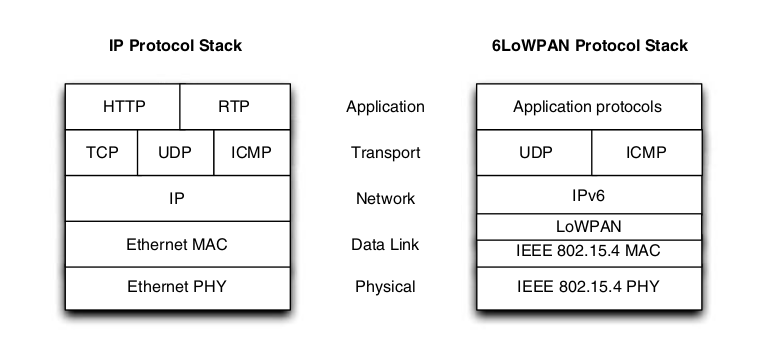
\includegraphics[width=0.8\linewidth]{ip_vs_low.png}
    \caption{IP and 6LoWPAN stack, see \cite[p.~16]{wie}}
    \label{fig:ip_vs_low}
  \end{figure}

  The IPv6 protocol stack with 6LoWPAN (sometimes called the 6LoWPAN protocol stack) is nearly 
  identical to a conventional IP stack, with a few notable differences. Primarily, 6LoWPAN only 
  supports IPv6, for which a small adaptation layer—the LoWPAN adaptation layer—has been defined 
  to optimize IPv6 for IEEE 802.15.4 and similar link layers, as detailed in \cite{rfc4944}. In practice, 
  many implementations of the 6LoWPAN stack in embedded devices combine the LoWPAN adaptation layer 
  with IPv6, allowing them to be displayed together as part of the network layer.

  The \gls{udp} \cite{rfc768} is the most commonly used transport protocol 
  with 6LoWPAN, and it can be compressed using the LoWPAN format. The \gls{tcp} is less frequently used due to concerns about performance, efficiency, and 
  complexity, although there have been recent efforts on guidance to use and implement TCP for the IoT \cite{rfc9006}. 
  The \gls{icmpv6} \cite{rfc4443} is utilized 
  for control messaging, including functions like \gls{icmp} echo requests, destination unreachable messages, 
  and Neighbor Discovery. While many application protocols are application-specific and in binary format, 
  there is a growing availability of more standardized application protocols.

\section{IEEE 802.15.4}
  Established by the IEEE, the IEEE 802.15.4 standards define low-power wireless radio techniques 
  and specify the physical and media access control layers that serve as the foundation for 6LoWPAN. 
  The IEEE 802.15.4-2011 version of the standards includes features such as access control via 
  CSMA/CA, optional acknowledgments for retransmission of corrupted data, and 128-bit  \gls{aes} encryption 
  at the link layer. It offers addressing modes that utilize both 64-bit and 16-bit addresses 
  with unicast and broadcast capabilities. The payload of a physical frame can reach up to 127 bytes, 
  with 72 to 116 bytes of the usable payload after link-layer framing, depending on different addressing 
  and security options \cite[Appendix B.1]{wie}.

  Star and point-to-point network topologies are supported by IEEE 802.15.4. The MAC layer can operate 
  with CSMA/CA in the beacon-less mode. In beacon-enabled mode, TDMA/TISCH for media access is utilized.
  The number of nodes, the length of the transmitted messages, and the level of radio interference 
  within the ISM band significantly influenced the average packet loss in IEEE 802.15.4 \cite{packet_loss}. 
  While the use of acknowledgments at the link layer enhances reliability, it complicates the 
  estimation of packet round-trip times.
\chapter{RIOT-OS and The GNRC Network Stack}
\section{RIOT Operating System}
  RIOT, the friendly operating system for the Internet of Things, is a real-time operating system,
  specifically designed for low-end IoT devices with a minimal memory in order of $\approx$ 10K Byte
  \cite{riot}. It can run on devices with neither memory management unit (MMU) nor memory protection unit (MPU).

  Under the distribution of LGPLv2.1 License, RIOT is free and open-source software, meaning it can
  be used and distributed by anyone. Furthermore, this license allows the linkage of RIOT with
  proprietary software and supports the ability to be customized by the end users.

  The design objectives of RIOT focus on several key areas: optimizing resource usage such as RAM, 
  ROM, and power consumption; supporting a broad spectrum of configurations, from 8-bit to 32-bit MCUs, 
  and accommodating various boards and use cases; reducing code duplication across different setups; 
  ensuring most of the code is portable across supported hardware; offering user-friendly software 
  platform; and enabling real-time capabilities. To realize these goals, one of the principles that
  the RIOT follows is modularity. 

  RIOT is organized into software modules that are combined at compile time, centered around a kernel 
  offering minimal functionality. This modular approach allows the system to be built in a way that includes 
  only the necessary modules for a given use case. As a result, both memory usage and system complexity 
  are kept to a minimum in practical deployments. The code structure of RIOT is illustrated in
  Figure \ref{fig:riot_code}:
  
  \begin{itemize}
    \item \textbf{core} provides the kernels and basic data structures like linked lists, LIFOs,
    and ringbuffers.
    \item Four parts of hardware abstractions:
      \begin{enumerate}
        \item \textbf{cpu} implements functionalities of microcontroller.
        \item \textbf{boards} selects, maps and configures the used CPU and drivers.
        \item \textbf{drivers} implement the device drivers.
        \item \textbf{periph} provides unified access to microcontroller peripherals and is used by
        device drivers.
      \end{enumerate}
    \item \textbf{sys} implements libraries beyond kernel features, such as cryptography, networking, and file
    system.
    \item \textbf{pkg} contains third-party libraries which do not exist within the main code 
    repository.
  \end{itemize}

  \begin{figure}[h]
    \centering
    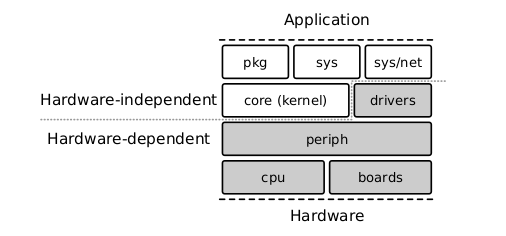
\includegraphics[width=0.8\linewidth]{riot_code}
    \caption{Structure elements of RIOT, see \cite[p.~3]{riot}}
    \label{fig:riot_code}
  \end{figure}

    Multi-threading is a builtin feature for RIOT to offer several benefits: (a) clear 
    logical separation between different tasks, (b) straightforward task prioritization, 
    and (c) easier integration of external code \cite[p.~4]{riot}. Various synchronization primitives, such
    as mutex, semaphore, and message passing (\textbf{msg}) are provided by RIOT kernel.
    Multi-threading can also be optional in the case of extremely low-memory usage of the application.

    RIOT's kernel employs a scheduler that uses fixed priorities and preemption with O(1) operations, 
    enabling soft real-time capabilities. Specifically, the time required to interrupt and switch 
    between threads is bounded by a small upper limit, as operations like context saving, selecting 
    the next thread, and context restoring are deterministic. The system follows a class-based 
    run-to-completion scheduling policy, where the highest-priority active thread is executed and 
    can only be interrupted by interrupt service routines (ISRs). This scheduler allows RIOT to 
    effectively prioritize tasks, ensuring that high-priority events can preempt lower-priority 
    tasks as needed.

    RIOT's scheduler operates in a tickless manner, meaning it does not rely on CPU time slices 
    or periodic system timer ticks. As a result, the system remains in a low-power state unless 
    an actual event occurs, such as an interrupt triggered by hardware. Wake-up events can be 
    initiated by a transceiver receiving a packet, timers expiring, buttons being pressed, or 
    similar activities. When no threads are in a running state and no interrupts are pending, 
    the system automatically switches to the idle thread, which has the lowest priority. 
    The idle thread, in turn, transitions the system into the most energy-efficient mode available 
    thereby reducing energy consumption.
\section{GNRC}
\subsection{Overview}
  - Design of the network stack
    
    - Northbound API with sock for application

    - Southbound API for network interface

  - Each network stack runs on its stack, communicate with each other through IPC api.
\subsection{The Packet Buffer - pktbuf}
  - The copy on write nature
  
  - Central packet buffer to reduce packet copy.
\subsection{GNRC's Module Registry - netreg}
  - What it is?
\subsection{A Common Inter-Modular API - netapi}
  - Does it still exist?
\subsection{Network Interfaces and Device Drivers}
  - Netif and how it works


\chapter{Concepts of Wireguard}
  This chapter provide the core concepts of Wireguard protocol, especially in its handshake
  and timer state machine. Section \ref{w1} gives a high-level overview of the traits of the
  protocols, and the cryptography primitives that they build upon. 
  Section \ref{w2}  details the fondational handshake protocol that Wireguard's
  key exchange protocol builds upon. Section \ref{w3} defined all messages types of Wireguard and
  section \ref{w4} descibes the timer state machine.
\section{Protocol \& Cryptography} \label{w1}
\subsection{Overview}
 Wireguard works as an encrypted IP network tunnel, resides at the layer 3 of the OSI layer, and
 uses UDP as its transport protocol. The establishment of a secure session before any 
 transmission of data is via 1-RTT key-exchange handshake protocols. This handshake protocol
 is designed based on a Trevor Perin's noise handshake pattern \cite{noise}. After the handshake, the  
 transported IP payload are protected using ChaCha20-Poly1305 Authenticated Encryption with 
 Associated Data (AEAD) \cite{rfc8439}.

 In Wireguard, the endpoints of communication have no role of server and client, but works in a
 peer-to-peer style. At any point in time, a peer can have a role of an \textbf{initator}, start to send 
 a handshake initiation message to create a secure channel with a \textbf{responder}. If the secure channel
 is not active for some amount of time, the initiator peer can change to a responder in the event of
 a the previous responder tries to initiate a new handshake, leading to the establishment of a new session
 between 2 peers. Figure \ref{fig:pwu_hs} illustrates this handshake flow with periodic key rotation.

\begin{figure}[h]
  \centering
  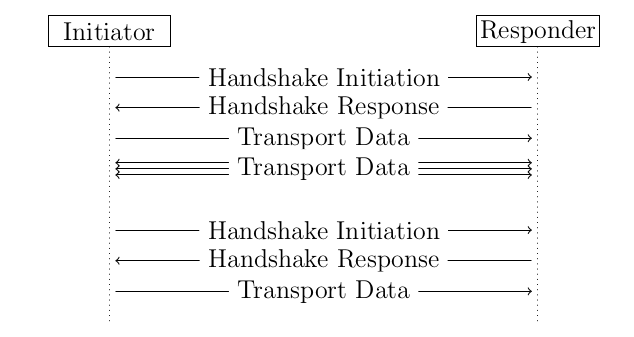
\includegraphics[width=0.8\linewidth]{pwu}
  \caption{After the handshake, both peers can send data towards each other. After a duration, rekeying occurs to create a new session. See \cite[p.~7]{pwu}}
  \label{fig:pwu_hs}
\end{figure}

 A static 32-byte Curve25519 \cite{curve} public key are used to identified an endpoint inside the tunnel. Without the
 proof of sender's knowledge on this public key, an endpoint will never respond. Thus, adversaries can't
 probe any system protected by Wireguard, using port scanning if they do not know the long-term static 
 public key.

The Wireguard handshake protocol can be considered as a 1.5 round-trip time (1.5-RTT) handshake \cite{pwu}. 
Upon the reception of the handshake response after sending a handshake initiation, the initiator
can promplty begin delivering encrypted payload. To safeguard against replay attacks, 
the responder must wait to send encrypted data messages until it has received an encrypted data 
message from the initiator, which serves as an acknowledgment of the handshake response.

During a handshake, new ephemeral key pairs will be generated by both parties, with the private key
being wiped after the handshake, assuring the forward secrecy of the session. Each session is bound
by fixed lifetime and the number of data messages that can be sent. When either of the limits is reached,
the derivation of new session keys are required if the peers want to extend the communication. The impact
of compromised session key is also mitigated by frequent periodic key rotation.

There is no direct shutdown signal within the protocol, only session removal after a fixed duration.
Even if one side has terminated its VPN tunnel, the peer would remain unaware and 
keep forwarding data.

Wireguard also provides an optional pre-shared symmetric key (PSK) mode, where any pairs of peer
pre-share a 256-bit symmetric encryption key between themselves, to assure the post-quantum 
security as long as the PSK never leaks out. This protection is against the idea that if 
adversaries may be recording all the traffic for a long time, until the quantum computer exists.
With PSK, despite the fact they maybe break all Curve25519-encrypted traffic, but not the ones that
include a PSK.

Another adversary model that Wireguard mititage is the denial of service through CPU exhaustion denial
of services attack \cite[p.~268]{cpu}. This mechanism is achieved via an encrypted cookie, when a peer is currently 
under load. This will be explained more in section \ref{iot:cookie}.

At last, Wireguard is cryptographically opinionated. The protocol intentionally does not provide 
any form of flexibility when it comes to choosing the cryptography suite, hence a negation for
cryptography algorithms does not exist. Specifically, Wireguard uses the following modern
cryptography constructions:
\begin{description}
  \item[Noise protocol framework]  A set of cryptographic handshake patterns that 
  serve as building blocks for creating new secure protocols with authenticated key agreement.
  \item[Elliptic Curve Diffie-Hellman (ECDH)] A Curve25519-based key-argeement protocol 
  with small key size and simple requirements regarding key validation.
  \item[ChaCha20-Poly1305] a modern AEAD combining ChaCha20 \cite{chacha20} stream cipher 
  and Poly1305 \cite{poly1305} authenticator to achieve authenticity and confidentiality. 
  \item[XChaCha-Poly1305] an extended version of chacha20-poly1305 that supports 192-bit nonce.
  This is used for cookie encryption \cite{irtf-cfrg-xchacha-03}.
  \item[HKDF] The HMAC-based Key Derivation Function \cite{rfc5869} to derive the encryption
  and decryption keys from the handshake state, keys and protocol messages.
  \item[BLAKE2] A fast and cryptographic hash function for message authentication code and is used
  by the HKDF \cite{rfc7693}.

\end{description}

\subsection{Cryptokey Routing}
  The binding between peers and the allowed source IP addresses is the fundamental principle to build 
  a secure VPN. As mentioned above, in Wireguard, peer must be identified by the 32-byte
  Curve25519 public key, allowing an association between the public key and the set
  of allowed IP addreses on the peer. This simple mapping is the concept behind the cryptokey
  routing table of Wireguard. A transmission of outbound packet will consult this table to search
  for the approriate public key, using the IP destination address of the packet. With inbound packets,
  after decryption and authentication, the source IP address need to be resolved to the same 
  peer that have the same public key used in the secure session for decrypting the packet. 
  In cryptokey routing table, each peer may optionally pre-specify an outer external IP address
  and UDP port of that peer's endpoint. If the endpoint is not specified, the external
  source IP of the machine will be used to determine the endpoint .
  This design also allow the peers to roam freely between different external IP addresses as the
  public is the main identification of the peer.
  
  Combining the roaming and the cryptokey routing table, when the network interface needs
  to send the data out, the flow start with the inspection of the IP destination of the packet 
  to find the corresponding peer and its public key (An ICMP "no route to host" will be returned
  in case of no peer). The packet is then encrypted with mentioned AEAD, prepended with
  extra headers and sent as a UDP packet to the internet. On the receiving flow, when a UDP packet
  is received, Wireguard finds the matching peer, decrypts the packet and updates the peers' endpoint.
  If the packet is either not an IP packet or there is no entry for source IP address of the packet
  inside the cryptokey routing table, the packet is droped. Otherwise, the packet will be dispatched
  to the layer above.
\section{Noise} \label{w2}
\section{Wireguard Messages} \label{w3}
\section{Timers} \label{w4}
\chapter{Wireguard and the IoT}
\subsection{Cryptography Resilience}
\section{Virtuous Silence}
\section{Stateful firewall}
\section{Cookies and Denial of Services Attack} \label{iot:cookie}
\section{Roaming \& NDP}
\chapter{Design and Implementation of Wireguard for GNRC}
This chapter covers the specific requirements for the Wireguard adaptation for GNRC, the design 
details to meet the requirements and important implementation aspects inside the Wireguard source
code for RIOT.
\section{Requirements}
  \begin{itemize}
    \item \textbf{Static memory allocation}: Dynamic memory allocation is prohibited within RIOT core 
    components to maintain a predictable runtime memory usage and real-time performance. With
    Wireguard being at the layer 3 of the network stack, the protocol must use static memory
    allocation exclusively.
    \item \textbf{Security}: The GNRC implementation needs to be align to the security properties that
    the original Linux implementation holds. This includes the resistant to replay attack and
    side-channel attack \cite{side}, perfect forward secrecy, low probability of handshake collision \cite{pwu}
    ,cryptographic soundness, and safety from concurrency bugs.
    \item \textbf{Interconnectiviy with other Wireguard implementation}: The RIOT adaptation must 
    be able to communicate with other RIOT Wireguard node and obviously the Linux implementation.
    \item \textbf{Integration to RIOT network interfaces API}: Similiar to the Linux implementation,
    Wireguard will be an network interface, receive IPv6 packets from the layer above, and
    hande the all the encryption and dispatching.
    \item \textbf{6LoWPAN compatiblility}: The Wireguard implementation only supports IPv6 packet
    to be compatible with the 6LoWPAN layer.
  \end{itemize}
\section{Event-driven architecture}
  Taking inspiration from BoringTun \cite{boringtun}, the Wireguard implementation handles
  packets and timers in an event-oriented manner. Three different kinds of event can occur within
  a Wireguard session:
  \begin{itemize}
    \item Transmitting data from the IP layer.
    \item Reception of a packet from any peer.
    \item The timeout event related to the Wireguard timers.
  \end{itemize}

  \begin{figure}[h]
    \centering
    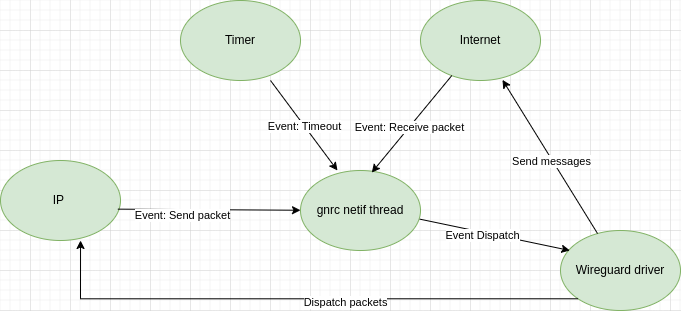
\includegraphics[width=\linewidth]{wireguard}
    \caption{GNRC Wireguard Software Architecture}
    \label{fig:wireguard}
  \end{figure}

  Figure \ref{fig:wireguard} illustrates the overview of the architecture of the GNRC Wireguard
  implementation. The Wireguard driver is the core component where it executes the Noise handshake,
  handles the functions triggered by the timeout event, encrypts, decrypts and transmits packet to
  the IP layer or the internet outside. To make use of the existing RIOT system, the GNRC netif's
  event queue is used as the central event listener for all 3 types of event. 
  
  Whenever, a packet is received on the UDP port of Wireguard, new event to handle the reception will be pushed
  at the netif's event queue, letting Wireguard make the decision whether to responde to 
  the peer if the packet is a handshake message, dispatch the packet directly to the IP layer if 
  it is authenticated or discard if the packet is invalid. 

  An IP layer will mostly be unaware of the inner working of Wireguard, as it will only transmit the
  packet to the specified netif and receives the pre-processed IPv6 packet from the driver. One thing
  to note is that the Linux implementation of Wireguard will queue the packets for another thread
  to process. The GNRC also follows that design, but with smaller packet queue to match the
  constrained environment.

  Every expiration of a timer, like timer for retransmission of the handshake or passing the
  keepalive, the event will also be pushed on top of the event queue for the driver to handle later.
  
  The design reduces the complexity of concurrency, as every event is handled sequentially, making it impossible for 
  other threads to
  meddle with the inner cryptography state of the driver. Although it could make the netif thread
  a bottleneck of performance, the thread would not be overload in a normal circumstance of
  IoT environment.

\section{Network Interfaces API}
  Show the supported API.

  create a netif thread like any other netif.
  
  Mention on the connect problem to start the handshake initation first. Disconnect will
  disconnect from a peer only. 

  Shutdown will clean all the peer state of Wireguard. 
  
  The netif peer contains the configuration of the peer on the Wireguard drivers.

  Init the peer with default configuration. Adding the peer is concurrently safe as with a 
  central lock around the list of peer. Allow
  to add the IPv6 address on a netif like a a normal netif would do.
\section{Memory allocation \& optmization}
  The number of peers must be preconfigured, hence the memory for peers are statically configured
  before hand. Peer that are freed marks with a boolean variable valid to known
  the peer is usable by other thread or not.

  Every search for keypair, generation of index or look up based on the index, allowed ip
  are linear iteration over all the peer.

  Instread of Making Wireguard running in its own thread, running in its own event loop
  with its own queue, Wireguard drivers run in the same thead as the netif, making 
  use of the existing netif event queue structure and msg box of netif to the handle.
  Although it enforces an order, however as the sending of packet should know beforehand
  to ensure the realtime cap, the packet queue won't be overload with the number of concurrent
  events.

  There is a packet queue, but only allows the total maximum of the number of peer multiplied by 2.
  This comes from the assumption is the device either send packet periodically, or sometimes
  do the sending. If the packet queue is full and there in no handshake session, the packet 
  is simply discarded.

  To reduce the fragmentation, the realloation and the merging of data happens only one during the final preparation
  of the transport message. The code is a follow, first we allocate enough space for the padded
  packet and the header. Then copy all the payload after the IPv6 to the end, then slide
  the orignal IPv6 header to its right place.

\section{Security Requirements \& Implementations}
  The packet is silently drop if it no valid. crypto{\_}secure{\_}wipe and crypto{\_}equals are used to
  handle the comparsion between the keypairs, and the wipe out of the packet state. ensuring
  there is no leaking.
  
  The ECDH implementation include an additional check for zero bytes to prevent the zero public 
  key.

  Less likey to have concurency bugs because of the sequential nature to handle all the noise 
  handshake. 

  Crypto primitve is implemented in the same way as the Linux does.

  Regarding the under load condition to prevent the DoS, seemly counter the number of event on the
  event queue, as it thread allow to hanle 16 events at once, the limitation of the number of
  event is 16 before handle the final handshake, instead sending out the cookie is 12 events at a time.
\section{Implementation Status}
  Finished features:
    handling of Noise handshake state 
    support of every wireguard messages.
    timer state machine
    packet queuing.

  functional enough to communicate with the Linux implementation.
  
  Missing features:
    private key configuration
    removal of peers

  Problems:
     on the neighbor cache entry to dispatcht the packet out, still required to install
     the entry to support sending to the endpoint. 
\chapter{Testing}
\section{Methodology}
\section{Environment}
\section{Scenario 1}
\section{Scenario 2}
\section{Scenario 3}
\section{Scenario 4}
\section{Memory Usage}

\chapter{Conclusion and Future Work}
  With more embedded device, the desire for security increased as well. This thesis
  provides an adaptation of a well-designed security protocols that show promising
  adaptation for the IoT worlds. The gnrc Wireguard implementation is functional
  whilst missing features on configuration to acutally be used in the production.

  Improvements can be maded to reduced the memory footprint, and power consumption
  of Wireguard. Further measurement and testing are required to ensure the correctness.
  Performance evaluation vs other security protoocls like DTLS and Diet-ESP, to
  present an overiew of how security protocols compete against each other.

\printbibliography[title={References}]

\end{document}